\chapter{ Specificarile aplicatiei}
\label{chap:ch5}

\par Pe partea de back end sunt prezente doua servere, unul scris in JavaScript cu ajutorul framework-ului Node js care serveste partea de front-end cu toate datele de care are nevoie si un server scris in Python cu ajutorul framework-ului Flask cu ajutorul caruia aflu filme recomandate pentru un film sau o lista  de filme.

\section{Baza de date}
\label{sec:ch5sec1}

\begin{figure}[htbp]
\centerline{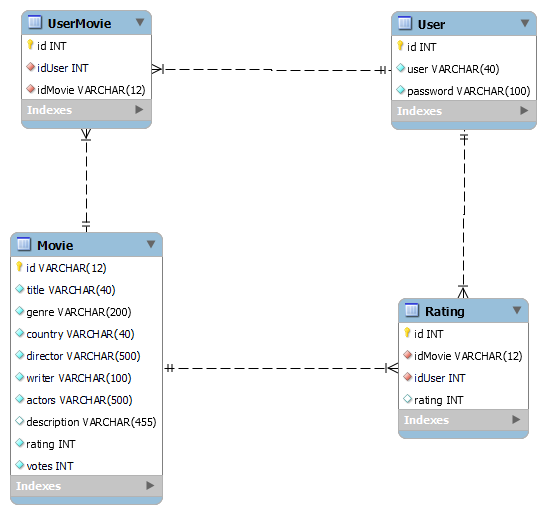
\includegraphics[width=10cm, height=10cm]{figures/diagrama db.png}}
\caption{Diagrama baza de date.}
\label{fig}
\end{figure}

\par Un lucru foarte important in dezvoltarea aplicatiei a fost alegerea bazei de date, am optat pentru pentru MySql versiunea 8.0. In tabelul de User voi salva datele de inregisrare a unui utilizator , in tabelul  Movie sunt prezente datele care descriu un film prin colloanele:title,genre,country,directors,writers,actors,description,votes si rating, in tabelul Rating salvez datele unui rating dat de un user pe laga valoare ratingului salvez si id-urile de la film si user pentru a stii cine da rating si la ce film totodata pe partea de back-end fac si o actualizare a rating ului si numarului de voturi din tabelul Movie asta pentru o a face aplicatia sa se miste mai rapid, iar in tabelul UserMovie salvez id ul de la un user si id ul de la un film reprezentand un film pe care utilizatorul l-a vizualizat.

\section{Server Node Js}
\label{sec:ch5sec1}

\par Serverul de Node Js este folosit pentru a se face inregistrare, login, returanrea tuturor filmelor care contin un numit sub titlu, adaugarea unui film la lista utilizatorului, returnarea a tuturor filmelor unui utilizator si adaugarea de rating a unui film. Cu ajutorul pachetului Express stabilesc rutele si pornesc serverul. Cand se face un request pe o ruta, se apeleaza functia asignata din Service, care are rol de a modela datele in functie de cum avem nevoie. Pentru a comunica cu baza de date ne folosim de Repository, acesta face legatura cu baza de date.
\par Standardul REST („representational state transfer”) a fost creat pentru a ghida design-ul și  arhitectura serviciilor web. REST descrie cum ar trebui să se comporte internetul. Orice serviciu care reușește să se încadreze în parametrii și regulile descrise de acest standard se numește un serviciu RESTful. Atunci când o cerere de client se face printr-un API RESTful, acesta transferă o reprezentare a 
stării resursei către solicitant sau punct final. Aceste informații sau reprezentări sunt livrate într-unul din mai multe formate prin HTTP: JSON (Javascript Object Notation), HTML, XLT, Python, PHP sau text simplu. JSON este cel mai popular limbaj de programare folosit, deoarece, în ciuda numelui său, este limbaj-agnostic, precum și lizibil atât de oameni, cât și de mașini.Altceva de reținut: anteturile și parametrii sunt, de asemenea, importanți în metodele HTTP ale unei cereri HTTP RESTful API, deoarece conțin informații importante de identificare referitoare la metadatele cererii, autorizarea, identificatorul uniform al resurselor (URI), cache, cookie-uri și 
Mai Mult. Există anteturi de solicitare și anteturi de răspuns, fiecare cu propriile informații de  conexiune HTTP și coduri de stare.
\par Serverul respectă standardul REST API. Crearea entităților se face cu PUT, interogările cu GET, ștergerea cu DELETE, iar restul operațiilor cu POST. Specificațiile API în format OpenAPI se pot găsi la documentație API

		\begin{figure}[htbp]
			\centerline{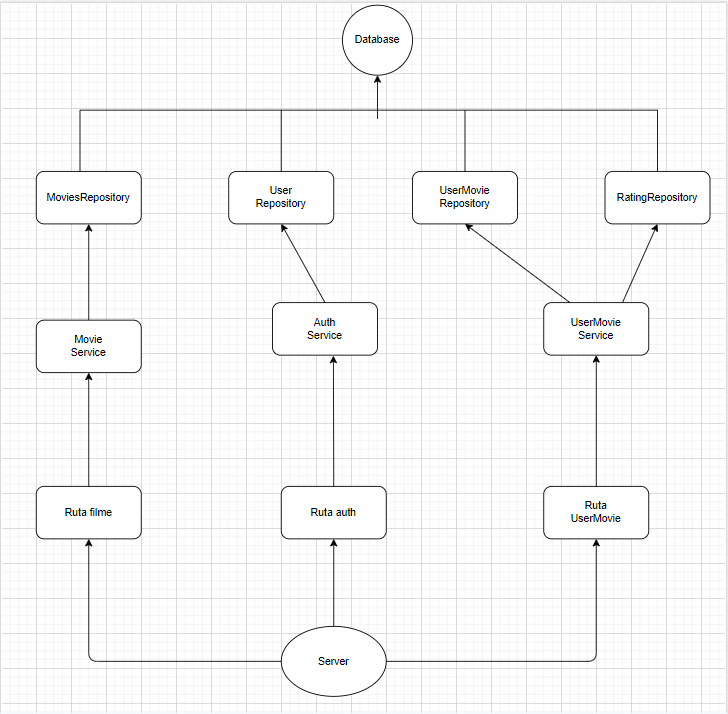
\includegraphics[width=13cm, height=10cm]{figures/diagrama clase node js.png}}
			\caption{Arhitectura server Node Js .}
			\label{fig}
		\end{figure}

\subsection{Inregistrare}
\par Procesul de inregistrare este unul simplu, pasii fiind urmatorii:
\begin{enumerate}
  	\item Se trimit datele catre server
  	\item Se valideaza datele primite 
 	\item Daca datele sunt valide se verifica daca numele utilizatorului se afla in baza de date deoarece numele trebuie sa fie unic pentru fiecare utiliztor
	\item Daca totul este bine pana la acest pas se face has la parola pentru o mai buna securitate
		\begin{figure}[htbp]
			\centerline{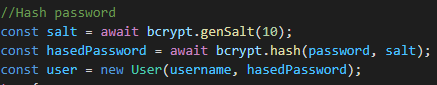
\includegraphics[width=15cm, height=4cm]{figures/hasparola.png}}
			\caption{Has la parola.}
			\label{fig}
		\end{figure}
	\item Următorul pas este de a apela functția din repositoy care adaugă un user in baza de date.
		\begin{figure}[htbp]
			\centerline{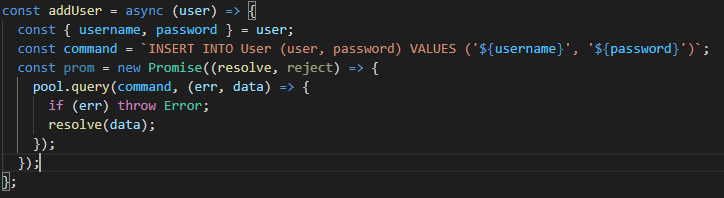
\includegraphics[width=19cm, height=6cm]{figures/adaugare user.png}}
			\caption{Adaugare user in baza de date.}
			\label{fig}
		\end{figure}	
	\item Dacă adăugarea s-a efectuat cu succes se returneaza un messaj de succes altfel se returnează un mesajul de eroare.
\end{enumerate}

\subsection{Autentificare}
\par Pașii pentru procesul de autentificare sunt următorii
\begin{enumerate}
  	\item Se trimit datele catre server
  	\item Se valideaza datele primite
  	\item Se verifica daca username-ul se afla in baza de date 
		\begin{figure}[htbp]
			\centerline{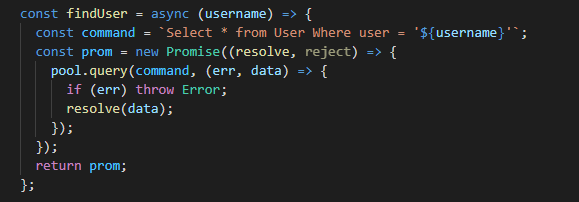
\includegraphics[width=19cm, height=6cm]{figures/cautare user.png}}
			\caption{Cautare dupa username in baza de date}
			\label{fig}
		\end{figure}	
	\item Daca se găsește user-ul in baza de date se verifică parola trimisă in requst cu cea din baza de date apoi se trimite raspunsul in functie de potrivirea celor doua parole, daca rapunsul este valid se va trimite id-ul user-ului care va reprezenta token-ul pentru front-end, daca  parolele nu corespund se va trimite status 400 si un mesaj de eroare.
		\begin{figure}[htbp]
			\centerline{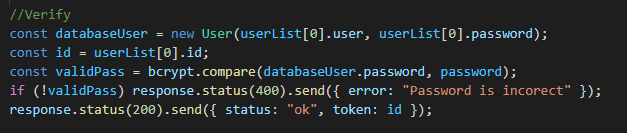
\includegraphics[width=19cm, height=6cm]{figures/verificare login.png}}
			\caption{Verificare parola si trimitere raspuns}
			\label{fig}
		\end{figure}	
\end{enumerate}


\subsection{Lista filmelor care contin un subtitlu}
\par Pașii pentru returnarea listii sunt:
\begin{enumerate}
  	\item Dupa se se apeleaza ruta specifica se ia din body titlul
  	\item Se apeleaza functioa din repository care returneaza lista
  	\item In repository se iau toate filmele din baza de date apoi se parcurg pentru a pastra doar filmele care contin subtitlul dat.
		\begin{figure}[htbp]
			\centerline{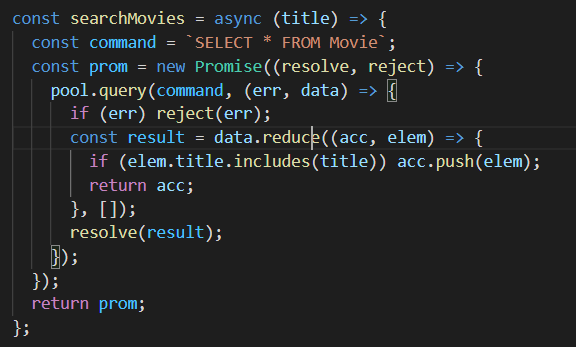
\includegraphics[width=19cm, height=6cm]{figures/cautarea filme.png}}
			\caption{Functia din repository care cauta filmele}
			\label{fig}
		\end{figure}	
			
\end{enumerate}

\subsection{Adaugarea unui film la lista}
\par Pașii pentru adaugare sunt:
\begin{enumerate}
  	\item Exista o ruta care trebuie sa primeasca intr-un body id-ul user-ului si id-ul unui film
  	\item Se apeleaza functia din service respectiva rutei
	\item Se adauga cele doua id uri in baza de date
  	\item In cazul unei erori se returneaza codul 400, iar daca totul s-a executat asa cum trebuie se returneaza codul 200 si statusul true.
		\begin{figure}[htbp]
			\centerline{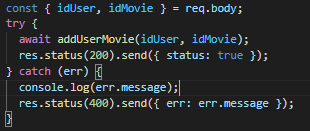
\includegraphics[width=10cm, height=6cm]{figures/adaugare film lista.png}}
			\caption{Functia pentru ruta de adaugat filme}
			\label{fig}
		\end{figure}	
	\item In cazul in care se doreste stergerea filmului respectiv din lista se apeleaza ruta "/del" cu cele 2 id-uri
\end{enumerate}


\subsection{Acordare rating}
\par Pașii pentru adaugare sunt:
\begin{enumerate}
  	\item Exista o ruta care trebuie sa primeasca intr-un body id-ul user-ului , nota data si id-ul filmului
  	\item Se apeleaza functia din service respectiva rutei
	\item Se adauga cele doua id uri si nota in baza de date 
	\item In baza de date cu filme se modifica la id-ul filmului: se incrementeaza cu unu numarul de votanti si se aduna la rating nota data, acest lucru ajuta la calcularea mediei generale a filmului fara a mai face un select cu toate notele unui film.
  	\item In cazul unei erori se returneaza codul 400, iar daca totul s-a executat asa cum trebuie se returneaza codul 200 si statusul true.
		\begin{figure}[htbp]
			\centerline{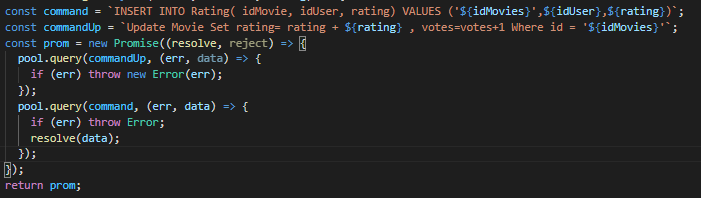
\includegraphics[width=15cm, height=5cm]{figures/functie rating.png}}
			\caption{Functia pentru ruta de adaugat filme}
			\label{fig}
		\end{figure}	
	\item In cazul in care se doreste stergerea filmului respectiv din lista se apeleaza ruta "/del" cu cele 2 id-uri
\end{enumerate}

\section{Server Flask}
\label{sec:ch5sec1}

\par Seveverul scris cu ajutorul framework-ului Flask este cel care face recomandari pentru un film sau pentru o lista de filme. La pornirea acestui server trebuie sa se stepte un anumit timp deoarece la pornire acesta ia toate datele de la baza de date apoi le proceseaza si calculeaza matricea de scoruri, face toate acestea pentru ca atunci cand un client cere recomandari pentru un film raspunsul sa fie minim si sa nu fie nevoie sa faca toate aceste calcule. Exista un dezanjantaj la aceasta metoda, daca intervin modificari la baza de date in acest timp nu  vor influenta scorurile, de exemplu daca un film va fi votat cu multe voturi nu se regasi in scorul final sau daca un film este sters din baza de date algoritmul din acest server inca il poate recomanda. Exista totusi variante pentru aceste probleme, se poate creea o functie care  sa reincarce datele iar la apelarea aceesteia sa se recalculeze matricele de scoruri, iar o a doua varianta putin mai neconvetionala se poate opri si reporni server ul acesta recalculand scorurile. Primul lucru pe care il face serverul dupa citire este procesarea datelor, dupa care creeaza sacul de cuvinte si vectorii care reprezinta filmele, urmatorul pas fiind calcularea scorului.Server-ul are doua rute una in care returneaza recomandaripentru un film si o ruta care returneza recomandari pentru o lista de filme.
\par Pentru a face recomandari pentru un film algoritumul ia din linia din matricea de scoruri cele mai mari n scoruri, n reprezentand numarul de filme pe care algoritmul trebuie sa il recomande, apoi returneaza o lista cu detaliile filmelor. Atunci cand se cere recomandari pentru o lista de filme algoritmul ia din matricea de scoruri mai multe filme pentru fiecare film, la final sortandu-le dupa scor si returneaza n filme cu cele mai bune scoruri. 
\begin{figure}[!h]
			\centerline{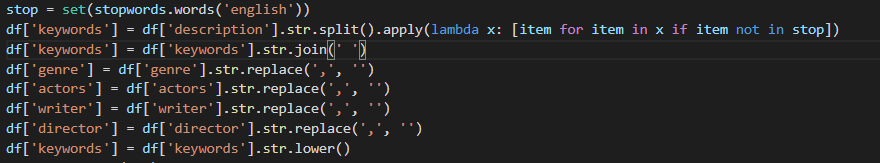
\includegraphics[width=15cm, height=6cm]{figures/prelucrare.png}}
			\caption{Prelucrarea datelor}
			\label{fig}
		\end{figure}

\begin{figure}[!h]
			\centerline{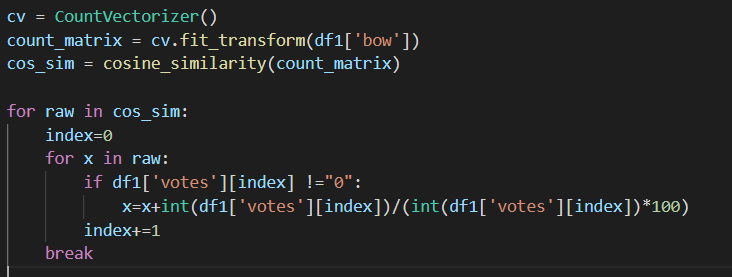
\includegraphics[width=15cm, height=6cm]{figures/calculare scoruri.png}}
			\caption{Calcularea matricii de scoruri}
			\label{fig}
		\end{figure}

\section{Front-end}
\label{sec:ch5sec1}

\par Front-endul este reprezentat de un site web scris cu ajutorul framework-ului React Js. Proiectul este impartit pe pagini care la randul lor contin diferite componente. Aceasta metoda a componentelor este foarte utila atunci cand se refoloseste cod, este ca si o functie care este scrisa o singura data dar este apelata in mai multe locuri. Exista doua tipuri de pagini, publice si private, cele publice pot fi accesate de un user fara a fi neoie de autentificare, iar cele publice necesita o autentificare. Stilizarea site-ului web se face cu ajutorul CSS-ului in doua moduri, una fiin prin importarea fisierelor de CSS in componente si pagini si una cu ajutorul injectarii in componente cu ajutorul JavaScript. Pentru a putea naviga intre pagini exista un router in care se specifica pentru fiecare ruta din aplicatie pagina care trebuie sa fie afisata si daca aceasta este publica sau privata, in cazul in care este privata iar user-ul nu s-a autentificat acesta va fi redirectionat la una din rutele publice. Acesta respectă standardul REST și se folosește de librăria axios pentru a face cereri către server.

\subsection{Autentificare si inregistrare}
\par Pașii sunt:

\begin{enumerate}
  	\item Atunci cand utilizatorul acceseaza site-ul web este redirectionat la pagina de autentificare unde trebuie sa introduca userul si parola
	\item Daca nu are un cont poate apasa re butonul de inregistrare unde va fi redirectionat catre pagina de inregistrare:
		\begin{enumerate}
		  	\item Dupa completarea folmularului de inregistrare si pasarea butonului datele vor fi validate
			\item Urmatorul pas este de a trimite datele la server
			\item Daca se primeste status 200 userv-ul va fi redirectionat catre pagina de autentificare
			\item Daca se primeste alt status se va afisa eroarea, iar pasii de inregistrare trebuie repetati pana se introduc date valide	
		\end{enumerate}
	\item Dupa ce toate datele de autentificare au fost introduse ele se trimit la server, iar daca datele sunt corecte se primeste ca si raspuns token-ul care fa fi salvat in memorie si utilizatorul va fi redirectionat catre pagina principala
	\item Daca de la server se primeste raspuns negativ se va afisa eroarea, iar pasii trebuie repetati.
\end{enumerate}